pdfoutput=1
\pdfoutput=1
% !TEX program = xelatex
\documentclass[12pt,a4paper]{article}
% ================================================================
% Packages
% ================================================================
\usepackage{amsmath,amssymb,amsthm}
\usepackage{mathtools}
\usepackage{bm}
\usepackage{graphicx}
\usepackage{hyperref}
\usepackage{geometry}
\usepackage{enumitem}
\usepackage{booktabs}
\usepackage{tikz}
\usepackage{tikz-cd}
\usepackage{xcolor}
\usepackage{cleveref}
\usepackage{bbm}
\usepackage{float}
\geometry{margin=2.5cm}
% ================================================================
% Hyperref setup
% ================================================================
\hypersetup{
    colorlinks=true,
    citecolor=blue,
    urlcolor=blue,
    pdfauthor={SCX},
    pdfsubject={SCX Hamiltonian Audit Theory},
% ================================================================
% Theorem environments
% ================================================================
\newtheorem{theorem}Theorem[section]
\newtheorem{lemma}[theorem]Lemma
\newtheorem{proposition}[theorem]{Proposition}
\newtheorem{corollary}[theorem]Corollary
\newtheorem{definition}[theorem]Definition
\newtheorem{conjecture}[theorem]Conjecture
\newtheorem{criterion}[theorem]{}
\theoremstyle{remark}
\newtheorem{remark}[theorem]Remark
\newtheorem{example}[theorem]Example
\newtheorem{protocol}[theorem]{}
% ================================================================
% Custom commands
% ================================================================
\newcommand{\R}{\mathbb{R}}
\newcommand{\C}{\mathbb{C}}
\newcommand{\Q}{\mathbb{Q}}
\newcommand{\Z}{\mathbb{Z}}
\newcommand{\F}{\mathbb{F}}
\newcommand{\N}{\mathbb{N}}
\newcommand{\A}{\mathcal{A}}
\newcommand{\E}{\mathbb{E}}
\newcommand{\Pbb}{\mathbb{P}}
\newcommand{\Var}{\mathrm{Var}}
\newcommand{\Cov}{\mathrm{Cov}}
\newcommand{\indep}{\perp\!\!\!\perp}
\newcommand{\loss}{\mathcal{L}}
\newcommand{\D}{\mathcal{D}}
\newcommand{\T}{\mathcal{T}}
\newcommand{\SCX}{\textsf{SCX}}
\newcommand{\RS}{\textsf{RS}}
\newcommand{\RSB}{\textsf{RSB}}
\newcommand{\oneRSB}{\textsf{1RSB}}
\newcommand{\fRSB}{\textsf{\infty RSB}}
\newcommand{\Parisi}{\textsf{Parisi}}
\DeclareMathOperator{\sgn}{sgn}
\DeclareMathOperator{\diag}{diag}
\DeclareMathOperator{\spec}{spec}
\DeclareMathOperator{\rank}{rank}
\DeclareMathOperator{\Tr}{Tr}
\DeclareMathOperator{\Auditable}{Auditable}
\DeclareMathOperator{\argmax}{arg\,max}
\DeclareMathOperator{\argmin}{arg\,min}
% Honest critique marker
\newcommand{\honestcrit}[1]{%
    \textcolor{red}{\textbf{[Honest Strike]#1}}%
% Proof-status markers
\newcommand{\rigorous}{\textnormal{\textbf{[Rigorous Proof]}}}
\newcommand{\heuristic}{\textnormal{\textbf{[Heuristic]}}}
\newcommand{\openproblem}{\textnormal{\textbf{[Open Problem]}}}
\newcommand{\honeststrike}{\textnormal{\textbf{[Honest Strike]}}}
% ================================================================
% Title
% ================================================================
\title{\textbf{Hamiltonian---}\\[4pt]
\large The Hamiltonian as an Audit Condition —\\[2pt]
Judging Auditability from the Energy Landscape}
\author{SCX}
\date{2026-6-30}
\begin{document}
\maketitle
\begin{center}
\footnotesize
\textbf{Version: } v1.0 \quad | \quad
\textbf{Status:} Preprint \quad | \quad
\textbf{Classification:} SCXTheoretical System — 
\end{center}
% ================================================================
% Abstract
% ================================================================
\begin{abstract}
SCXHamiltonian\textbf{}.
$\Auditable(\text{claim}) \Longleftrightarrow \Sigma_0 \leq \frac{1}{N}\log(M_{\min}/C)$, 
$\Sigma_0$awaiting.
$\RS$(), $\oneRSB$(), $\fRSB$()---
$T$.
$\RS$($\Sigma_0$, ), 
Distillation$\oneRSB$($\Sigma_0$, ), 
Distillation$\fRSB$($\Sigma_0$Growth, Galois).
\textbf{Keywords: } Hamiltonian; ; Parisi; ; Distillation; SCX
\end{abstract}
\tableofcontents
\newpage
% ================================================================
% 1. Introduction
% ================================================================
\section{:}
\subsection{SCXHamiltonian}
SCXHamiltonian~\cite{scx_hamiltonian}, : 
$\loss(\theta)$, Hamiltonian
$H(\theta) = \loss(\theta) + \frac{1}{\beta}\log Z(\beta)$$Z(\beta) = \int \exp(-\beta \loss(\theta))d\theta$
.$M$SCXHamiltonian$M$, 
, $M \to \infty$.
Core\textbf{}---SCX, 
Proof$M_{\min} \propto \exp(N\Sigma_0(e_\beta))$: 
\textbf{---.}"SCX", 
\begin{center}
\fbox{\parbox{0.85\textwidth}{
\centering
\textbf{, SCX, \\
\end{center}
\textbf{Hamiltonian}(Hamiltonian Pre-Audit Diagnosis)Core.
\subsection{?}
\begin{enumerate}[label=(\arabic*),itemsep=3pt]
    \item \textbf{SCX: } $M$, , ---, .
    \item \textbf{: } SCX, .
    \item \textbf{Distillation: } Distillation(Distillation)(Galois~\cite{scx_galois}DistillationHallucination~\cite{scx_distillation_hallucination}), \textbf{}.
\end{enumerate}
: \textbf{, Hamiltonian, .}
\subsection{}
\begin{enumerate}[label=(\arabic*),itemsep=3pt]
    \item 2: ---.
    \item 3: Parisi---RS$\fRSB$.
    \item 4: ---.
    \item 5: DistillationHamiltonian---Distillation.
    \item 6: ---HamiltonianStatus.
    \item 7: Honest Strike---Hamiltonian.
\end{enumerate}
% ================================================================
% 2. Audit Condition Theorem
% ================================================================
\section{}
\subsection{}
SCXHamiltonian~\cite{scx_hamiltonian}.
$M_{\min}$$\Sigma_0(e_\beta)$: 
\begin{equation}\label{eq:central_original}
    M_{\min}(\beta, \varepsilon) \geq C \cdot \frac{\exp(N \Sigma_0(e_\beta))}{-\log(1 - \varepsilon)} \cdot \left(1 + \mathcal{O}\left(\frac{1}{\sqrt{N}}\right)\right)
\end{equation}
$N$, $\Sigma_0(e_\beta)$$e_\beta$(), 
$C$, $\varepsilon$.
\textbf{}.
\begin{definition}[]
$M_{\text{feasible}}$.
\textbf{}, $\varepsilon$$\delta$SCX, 
$M_{\min} \leq M_{\text{feasible}}$.
\end{definition}
\begin{theorem}[ --- ]\label{thm:audit_condition_1}
Hamiltonian$H(\theta)$$\beta$$\Sigma_0(e_\beta)$.
\begin{equation}\label{eq:audit_condition}
    \boxed{\Auditable(\text{claim}) \;\Longleftrightarrow\; \Sigma_0(e_\beta) \leq \frac{1}{N} \log\left(\frac{M_{\text{feasible}} \cdot (-\log(1-\varepsilon))}{C}\right)}
\end{equation}
awaiting, \textbf{}: 
\begin{equation}\label{eq:threshold}
    \Sigma_0^{\text{crit}} = \frac{1}{N} \log\left(\frac{M_{\text{feasible}}}{C}\right)
\end{equation}
\begin{equation}\label{eq:audit_simple}
    \boxed{\Auditable(\text{claim}) \;\Longleftrightarrow\; \Sigma_0(e_\beta) \leq \Sigma_0^{\text{crit}} + \frac{1}{N}\log(-\log(1-\varepsilon))}
\end{equation}
\end{theorem}
\begin{proof}
\eqref{eq:central_original}$\Sigma_0$.
\begin{align}
    M_{\text{feasible}} &\geq M_{\min} \geq C \cdot \frac{\exp(N \Sigma_0)}{-\log(1-\varepsilon)} \\
    \exp(N \Sigma_0) &\leq \frac{M_{\text{feasible}} \cdot (-\log(1-\varepsilon))}{C} \\
    \Sigma_0 &\leq \frac{1}{N} \log\left(\frac{M_{\text{feasible}} \cdot (-\log(1-\varepsilon))}{C}\right)
\end{align}
$N \to \infty$, $\frac{1}{N}\log(-\log(1-\varepsilon))$, 
$\Sigma_0 \leq \Sigma_0^{\text{crit}}$.
$\hfill \square$
\end{proof}
\subsection{}
\begin{enumerate}[label=(\arabic*),itemsep=3pt]
    \item \textbf{$\Sigma_0$---"": } ($\Sigma_0$), , .
    \item \textbf{$\Sigma_0^{\text{crit}}$---"": } $M_{\text{feasible}}$, , .
    \item \textbf{awaiting: } $\Sigma_0$$\Sigma_0^{\text{crit}}$, ---.
\end{enumerate}
\begin{proposition}[$N$]\label{prop:large_N}
$N \to \infty$, : 
\begin{equation}
    \lim_{N \to \infty} \Pbb(\text{}) = \begin{cases}
        1, & \Sigma_0 < \Sigma_0^{\text{crit}} \quad \text{()} \\
        0, & \Sigma_0 > \Sigma_0^{\text{crit}} \quad \text{()}
    \end{cases}
\end{equation}
$N$, , $\sim \mathcal{O}(N^{-1/2})$.
\end{proposition}
\subsection{$\Sigma_0$}
$\Sigma_0(e_\beta)$.: 
\begin{enumerate}[label=\textbf{ \arabic*},leftmargin=*,itemsep=4pt]
    \item \textbf{Kac-Rice(): } Kac-Rice~\cite{fyodorov2004}: 
    \begin{equation}\label{eq:kac_rice}
        \Sigma(e) = \lim_{N\to\infty} \frac{1}{N} \log \E_\theta\left[|\det \mathcal{H}(\theta)| \cdot \delta(\nabla \loss(\theta)) \cdot \delta(\loss(\theta) - N e)\right]
    \end{equation}
    $\Sigma_0(e)$, Hessian$\mathcal{H}(\theta) \succeq 0$.
    \item \textbf{Hessian(): } , SGDHessian, 
    $f_{\text{neg}}$.: 
    \begin{equation}
        \hat{\Sigma}_0(e) \approx \frac{1}{N} \log \left(\frac{\#\{\text{}e\text{Hessian}\}}{\#\{\text{}\}}\right) + \text{}
    \end{equation}
    \item \textbf{(): } $M$$Q_{ab} = \frac{1}{N}\theta_a \cdot \theta_b$, 
    $\RSB$., $\rho(\lambda)$$\lambda \to 0$()
\end{enumerate}
% ================================================================
% 3. Parisi Breaking as Unauditability Criterion
% ================================================================
\section{Parisi}
\subsection{}
2\textbf{}---.
, \textbf{}---.
, \textbf{Parisi}~\cite{parisi1979,parisi1980,mezard1987}.
SCX, Parisi~\cite{scx_hamiltonian,scx_galois}, 
$\Sigma_0$.
\begin{definition}[Parisi---]
$M$()$Q_{\alpha\beta} = \frac{1}{N}\theta_\alpha \cdot \theta_\beta$.
$M \to \infty$, Parisi$q(x)$($x \in [0,1]$, ): 
\begin{equation}
    P(q) = \frac{dx}{dq}, \quad q = q(x)
\end{equation}
$q(x)$: Parisi$x$, $q(x)$.
$q(x)$""RSB.
\end{definition}
\subsection{: RS / 1RSB / $\infty$RSB}
\begin{criterion}[Parisi --- ]\label{crit:parisi}
Hamiltonian$T = 1/\beta$Parisi$q(x)$.: 
\begin{enumerate}[label=\textbf{(\arabic*)},leftmargin=*,itemsep=6pt]
    \item \textbf{$\RS$()--- : }
    $q(x) = q$().(), .
    \textit{: } $Q_{\alpha\beta}$, Marchenko-Pastur.
    $\Sigma_0 \approx 0$.
    \item \textbf{$\oneRSB$()--- : }
    $q(x) = q_0$($x < m$), $q(x) = q_1$($x > m$), $q_0 < q_1$, $m$Parisi.
    (), , .$K \propto 1/m$.
    :  $\to$ .
    \textit{: } $K$($K$), 
    Parisi$m$.$\Sigma_0 > 0$(Scale).
    \item \textbf{$\fRSB$()--- : }
    $q(x)$$[0,1]$.\textbf{}---, , ad infinitum.
    \textbf{}---Conclusion.
    \textit{: } Gap, Wigner.
    $\Sigma_0$Scale.
    Galois~\cite{scx_galois}$\fRSB$: 
    $\mathfrak{G}_{\text{audit}} \cong S_M$(), 
    $A_5$, .
\end{enumerate}
\end{criterion}
\begin{theorem}[Parisi-]\label{thm:parisi_audit}
\begin{enumerate}[label=(\arabic*),itemsep=3pt]
    \item $\RS \Longleftrightarrow$  $\Longleftrightarrow$  $\Longleftrightarrow$  $\Longleftrightarrow$ 
    \item $\oneRSB \Longleftrightarrow$  $\Longleftrightarrow$  $\Longleftrightarrow$  $\Longleftrightarrow$ 
    \item $\fRSB \Longleftrightarrow$  $\Longleftrightarrow$ Disagreement $\cong S_M$() $\Longleftrightarrow$ $A_5$ $\Longleftrightarrow$ Galois $\Longleftrightarrow$ 
\end{enumerate}
\end{theorem}
\begin{proof}[Proof Sketch]
\textbf{(RSB $\to$ ): } ~\cite{mezard1987}, 
Parisiawaiting""(valley-within-valley).
$\RS$; $\oneRSB$; $\fRSB$.
\textbf{( $\to$ Disagreement): }
$\RS$, ---; 
$\oneRSB$, ---; 
$\fRSB$, ---.
\textbf{( $\to$ Galois): }
$Q_{\alpha\beta}$(scx\_hamiltonian5.3~\cite{scx_hamiltonian}).
$\fRSB$, , $\mathfrak{G}_{\text{audit}}$, 
$\mathfrak{G}_{\text{audit}} \cong S_M$.$M \geq 5$, $A_5 \leq S_M$, Galois~\cite{scx_galois}, 
.$\hfill \square$
\end{proof}
\begin{remark}[RSB$\Sigma_0$]
$\Sigma_0$(2)RSB(): 
\begin{itemize}[itemsep=3pt]
    \item $\Sigma_0$\textbf{}---.
    \item RSB\textbf{}---.
\end{itemize}
$\Sigma_0$(), $\fRSB$()---.
: $\Sigma_0$$\RS$(, ).
\end{remark}
\subsection{Parisi}
\begin{table}[H]
\centering
\caption{Parisi}
\label{tab:parisi_params}
\begin{tabular}{@{}p{2.5cm} p{3.5cm} p{3.5cm} p{4.5cm}@{}}
\toprule
\textbf{Parisi} & \textbf{} & \textbf{} & \textbf{} \\
\midrule
$q(x)$ &  &  & $P(q)$ \\
$q(0) = q_{\min}$ &  & Disagreement & $\min_{\alpha \neq \beta} Q_{\alpha\beta}$ \\
$q(1) = q_{\max}$ &  &  & $\frac{1}{N}\|\theta_\alpha\|^2$ \\
$m$()&  & $K \approx 1/m$ &  \\
$x_{\max}$($\fRSB$)& $q(x)$ &  &  \\
\bottomrule
\end{tabular}
\end{table}
% ================================================================
% 4. Auditable Temperature Phase Diagram
% ================================================================
\section{}
\subsection{}
SCXHamiltonian, $\beta = 1/T$"": 
$\beta$(); $\beta$().
, $T$\textbf{}---(""), 
\begin{definition}[]
Hamiltonian$H(\theta)$, : 
\begin{itemize}[itemsep=3pt]
    \item \textbf{$T_f$: } , $\RS$.
    \item \textbf{$T_d$: } awaiting.
    \item \textbf{$T_c$(= Kauzmann$T_K$): } $\Sigma_0$($\Sigma_0(T_c) = 0$), Status.
\end{itemize}
: $T_f > T_d > T_c$()~\cite{mezard1987}.
\end{definition}
\begin{theorem}[]\label{thm:phase_diagram}
$T$: 
\begin{enumerate}[label=(\arabic*),itemsep=3pt]
    \item \textbf{$T > T_d$ --- (/): }
    , ($\Sigma_0 \to 0$).
    $\RS$.---.
    \item \textbf{$T_c < T < T_d$ --- (/$\oneRSB$): }
    .$\oneRSB$---.
    $\Sigma_0 > 0$.$M_{\min}$Scale.
    \item \textbf{$T < T_c$ --- (/): }
    .$\fRSB$---awaiting.
    $\Sigma_0$Growth, .
\end{enumerate}
\end{theorem}
\begin{figure}[H]
\centering
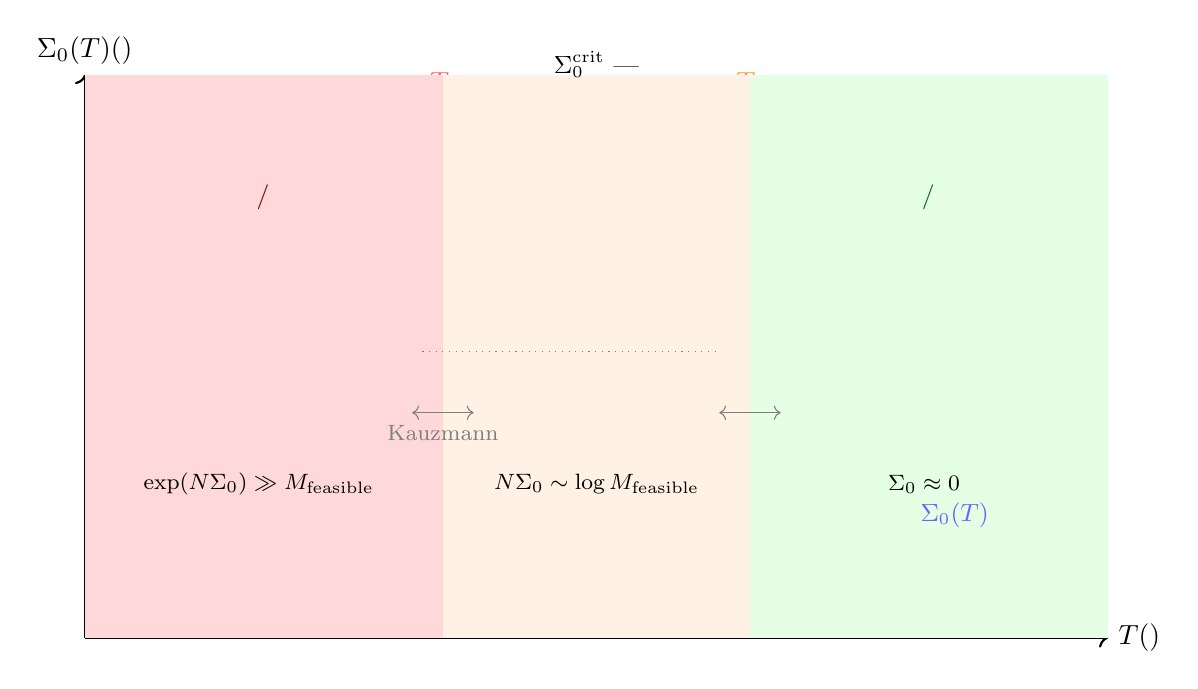
\begin{tikzpicture}[scale=1.3]
    % Temperature axis
    \draw[->,thick] (0,0) -- (10,0) node[right] {$T$()};
    \draw[->,thick] (0,0) -- (0,5.5) node[above] {$\Sigma_0(T)$()};
    % Complexity curve
    \draw[thick,blue!60] (0.5,4.8) .. controls (2,4.5) and (4,3.5) .. (5.5,2)
        .. controls (6.5,1) and (8,0.3) .. (9.5,0.05);
    % Phase boundaries
    \draw[dashed,red!60,thick] (3.5,0) -- (3.5,5.2) node[above,red!60] {$T_c$};
    \draw[dashed,orange!80,thick] (6.5,0) -- (6.5,5.2) node[above,orange!80] {$T_d$};
    % Phase labels
    \fill[red!15] (0,0) rectangle (3.5,5.5);
    \fill[orange!10] (3.5,0) rectangle (6.5,5.5);
    \fill[green!10] (6.5,0) rectangle (10,5.5);
    \node[red!70!black,font=\large\bfseries] at (1.7,4.8) {};
    \node[red!50!black,font=\small] at (1.7,4.3) {$\fRSB$ / };
    \node[orange!80!black,font=\large\bfseries] at (5,4.8) {};
    \node[orange!60!black,font=\small] at (5,4.3) {$\oneRSB$};
    \node[green!50!black,font=\large\bfseries] at (8.2,4.8) {};
    \node[green!40!black,font=\small] at (8.2,4.3) {$\RS$ / };
    % Annotations
    \node[blue!60,font=\small] at (8.5,1.2) {$\Sigma_0(T)$};
    \node[font=\small] at (5,5.6) {$\Sigma_0^{\text{crit}}$ --- };
    \draw[dotted,gray] (3.3,2.8) -- (6.2,2.8);
    \node[gray,font=\footnotesize] at (8,2.8) {};
    \node[align=left,font=\footnotesize] at (1.7,1.5) {$\exp(N\Sigma_0) \gg M_{\text{feasible}}$};
    \node[align=left,font=\footnotesize] at (5,1.5) {$N\Sigma_0 \sim \log M_{\text{feasible}}$};
    \node[align=left,font=\footnotesize] at (8.2,1.5) {$\Sigma_0 \approx 0$};
    % Phase transition arrow annotations
    \draw[<->,gray,thin] (3.2,2.2) -- (3.8,2.2);
    \node[gray,font=\footnotesize] at (3.5,2.0) {Kauzmann};
    \draw[<->,gray,thin] (6.2,2.2) -- (6.8,2.2);
    \node[gray,font=\footnotesize] at (6.5,2.0) {};
\end{tikzpicture}
\caption{.$T$(---"/""/"),}}$$M_{\text{feasible}}$.}
\label{fig:phase_diagram}
\end{figure}
\subsection{}
\textbf{}: 
\begin{proposition}[]\label{prop:heating}
()Status$\fRSB$, 
\textbf{}(, , )
$T_c$$\oneRSB$$T_d$$\RS$.
, \textbf{}---.
\end{proposition}
\begin{corollary}[-]
\begin{equation}
    \text{}(\text{}, \RS) \;<\; \text{}(\text{}, \oneRSB) \;<\; \text{}(\text{}, \fRSB)
\end{equation}
$T_d$---, $\RS$, , .
\end{corollary}
% ================================================================
% 5. Distillation Model Diagnosis
% ================================================================
\section{DistillationHamiltonian}
\subsection{Knowledge Distillation}
Knowledge Distillation~\cite{hinton2015distilling}---""""---
Perspective\textbf{}.
\begin{definition}[DistillationHamiltonian]
Teacher Model$T_\phi$($\phi$), Student Model$S_\theta$($\theta$).
Distillation: 
\begin{equation}\label{eq:distill_loss}
    \loss_{\text{distill}}(\theta) = \alpha \cdot \loss_{\text{CE}}(S_\theta(x), y) + (1-\alpha) \cdot \loss_{\text{KL}}(S_\theta(x) \| T_\phi(x))
\end{equation}
$\alpha \in [0,1]$, $\loss_{\text{CE}}$Entropy, $\loss_{\text{KL}}$KL.
DistillationHamiltonian: 
\begin{equation}\label{eq:distill_hamiltonian}
    H_{\text{distill}}(\theta; \phi) = \loss_{\text{distill}}(\theta) + \frac{1}{\beta} \log Z_{\text{distill}}(\beta)
\end{equation}
$\phi$Distillation\textbf{}(), .
\end{definition}
\subsection{Distillation}
\begin{theorem}[Distillation]\label{thm:distill_degradation}
DistillationConfigurationHamiltonian: 
\begin{enumerate}[label=\textbf{Configuration \arabic*},leftmargin=*,itemsep=8pt]
    \item \textbf{(Distillation): }
    \begin{itemize}[itemsep=2pt]
        \item \textbf{Hamiltonian: } $\loss(\theta)$Entropy, Distillation.
        \item \textbf{Parisi: } $\RS$().
        \item \textbf{: } $\Sigma_0 \approx 0$(, ).
        \item \textbf{Conclusion: } \textcolor{green!60!black}{\textbf{.}}
        \item \textbf{: } , .
    \end{itemize}
    \item \textbf{Distillation: }
    \begin{itemize}[itemsep=2pt]
        \item \textbf{Hamiltonian: } $\loss_{\text{distill}}(\theta)$$T_\phi(x)$
        \item \textbf{Parisi: } $\oneRSB$().
        \item \textbf{: } $\Sigma_0 > 0$, Distillation.
        \item \textbf{Conclusion: } \textcolor{orange}{\textbf{.}}
        \item \textbf{: } ""---
    \end{itemize}
    \item \textbf{Distillation(, Distillation): }
    \begin{itemize}[itemsep=2pt]
        \item \textbf{Hamiltonian: } Distillation.
        $k$Distillation: 
        \begin{equation}
            \loss^{(k)}(\theta) = \loss_{\text{CE}} + \sum_{j=1}^{k} \gamma_j \cdot \loss_{\text{KL}}(S_\theta \| S^{(j-1)})
        \end{equation}
        $S^{(j)}$$j$Student Model.\textbf{}.
        \item \textbf{Parisi: } $\fRSB$().
        \item \textbf{: } $\Sigma_0$Growth---Distillation.
        \item \textbf{Conclusion: } \textcolor{red}{\textbf{(Galois).}}
        \item \textbf{: } Distillation\textbf{}---
        $\fRSB$~\cite{mezard1987}.
        Teacher ModelStudent Model, 
        $k$"".
        , $S_M$, 
        Galois~\cite{scx_galois}.
        DistillationHallucination~\cite{scx_distillation_hallucination}ProofHallucination, 
        : Hallucination$\fRSB$.
    \end{itemize}
\end{enumerate}
\end{theorem}
\begin{proof}[Proof Sketch --- Configuration3(Distillation)$\fRSB$]
\heuristic ParisiProofDistillation$\fRSB$.
$j$DistillationKL$\loss_{\text{KL}}(S_\theta \| S^{(j-1)})$
$S^{(j-1)}$Configuration\textbf{}..
: $j$\textbf{}---$j-1$.
Parisi"$x$".
$k$, $k$.
$k \to \infty$($k$), 
$q(x)$$[0,1]$---$\fRSB$.
, Distillation, $j$$j-1$, 
\textbf{}(Branching Random Walk)~\cite{derrida1986}, 
.$\hfill \square$
\end{proof}
\subsection{Distillation}
\begin{figure}[H]
\centering
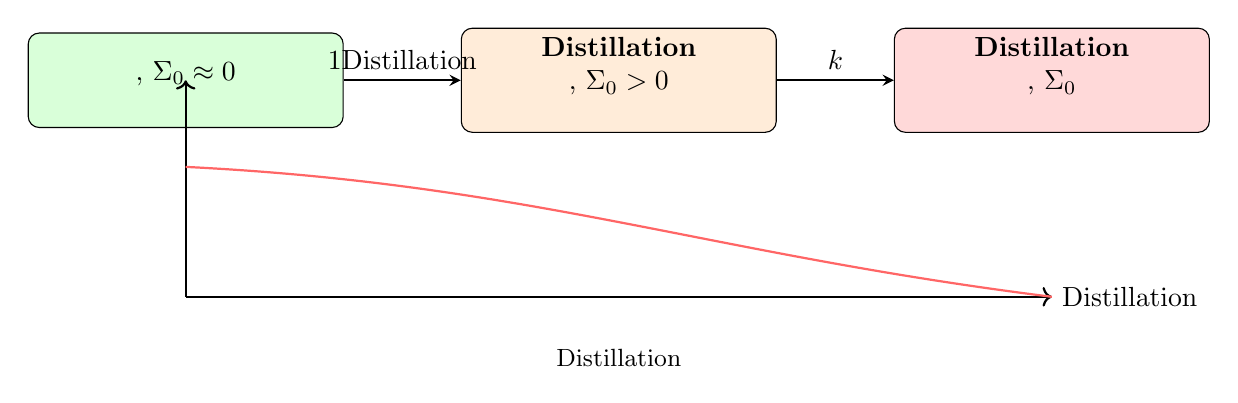
\begin{tikzpicture}[scale=1.1,
    box/.style={draw,rounded corners,minimum width=4cm,minimum height=1.2cm,align=center,fill=#1!15},
    arrow/.style={->,thick,>=stealth}]
    % Three boxes
    \node[box=green] (orig) at (0,0) {
        \textbf{}\\
        $\RS$, $\Sigma_0 \approx 0$\\
        \textcolor{green!60!black}{}
    };
    \node[box=orange] (once) at (5,0) {
        \textbf{Distillation}\\
        $\oneRSB$, $\Sigma_0 > 0$\\
        \textcolor{orange}{}
    };
    \node[box=red] (loop) at (10,0) {
        \textbf{Distillation}\\
        $\fRSB$, $\Sigma_0$\\
        \textcolor{red}{}
    };
    % Arrows
    \draw[arrow] (orig) -- (once) node[midway,above] {1Distillation};
    \draw[arrow] (once) -- (loop) node[midway,above] {$k$};
    % Degradation curve below
    \draw[->,thick] (0,-2.5) -- (10,-2.5) node[right] {Distillation};
    \draw[->,thick] (0,-2.5) -- (0,0) node[above] {};
    \draw[thick,red!60] (0,-1) .. controls (4,-1.2) and (6,-2) .. (10,-2.5);
    \node[font=\small,align=center] at (5,-3.2) {Distillation};
    % Annotations on phases
    \node[font=\footnotesize,green!60!black] at (1.5,-1.5) {$\RS$};
    \node[font=\footnotesize,orange] at (5.5,-1.7) {$\oneRSB$};
    \node[font=\footnotesize,red] at (8.5,-2.2) {$\fRSB$};
\end{tikzpicture}
\caption{Distillation.:}
\label{fig:distill_degradation}
\end{figure}
\subsection{DistillationHallucination}
DistillationHallucination~\cite{scx_distillation_hallucination}, ProofDistillationCompactnessHallucination.
Hamiltonian\textbf{}: 
\begin{proposition}[HallucinationHamiltonian]\label{prop:hallucination_origin}
DistillationHallucination$\fRSB$: 
\begin{enumerate}[label=(\arabic*),itemsep=3pt]
    \item \textbf{: } $\fRSB$, .
    \item \textbf{: } $\fRSB$, Phase Space().
    \item \textbf{: } $\fRSB$($\RS$$\oneRSB$), 
\end{enumerate}
\end{proposition}
% ================================================================
% 6. Operational Protocol
% ================================================================
\section{: Hamiltonian}
\subsection{}
: \textbf{SCX, /.}
\begin{protocol}[Hamiltonian]\label{prot:diagnosis}
\textbf{: } $f_\theta$($\theta \in \R^N$), $\D_{\text{train}}$, $\D_{\text{val}}$, 
$M_{\text{feasible}}$, $\{T_1, T_2, \ldots, T_K\}$.
\textbf{: } ($\{\text{}, \text{}, \text{}\}$).
\end{protocol}
\subsection{}
\begin{enumerate}[label=\textbf{ \arabic*},leftmargin=*,itemsep=8pt]
    \item \textbf{: }
    \begin{itemize}[itemsep=2pt]
        \item $R$, SGD()$\D_{\text{train}}$, $R$Configuration$\{\theta_r\}_{r=1}^{R}$($R \geq 100$).
        \item $e_r = \loss(\theta_r)$.
        \item (): 
        \begin{equation}
            Q_{rs} = \frac{1}{N} \frac{\theta_r \cdot \theta_s}{\|\theta_r\| \|\theta_s\|}, \quad r,s = 1,\ldots,R
        \end{equation}
    \end{itemize}
    \item \textbf{Hessian: }
    \begin{itemize}[itemsep=2pt]
        \item $\theta_r$, Hessian$\mathcal{H}(\theta_r) = \nabla^2_\theta \loss(\theta_r)$$k$(Lanczos, $k \sim 100\text{--}500$).
        \item $f_{\text{neg}}^{(r)}$$\lambda_{\min}^{(r)}$.
        \item Verdict: $f_{\text{neg}}^{(r)} > 0$, ---.
    \end{itemize}
    \item \textbf{$\Sigma_0$: }
    \begin{itemize}[itemsep=2pt]
        \item HessianConfiguration($\lambda_{\min} \geq -\epsilon$, $\epsilon$).
        \item Configuration$e$, Configuration$\mathcal{N}(e)$.
        \item : 
        \begin{equation}
            \hat{\Sigma}_0(e) = \frac{1}{N} \log \mathcal{N}(e) - \frac{1}{N} \log R + \text{Jacobi}
        \end{equation}
        \item : $\hat{\Sigma}_0(e_\beta) \leq \Sigma_0^{\text{crit}}$?(~\ref{thm:audit_condition_1})
    \end{itemize}
    \item \textbf{RSBVerdict: }
    \begin{itemize}[itemsep=2pt]
        \item $R \times R$$Q_{rs}$$\{\lambda_1 \geq \lambda_2 \geq \cdots \geq \lambda_R\}$.
        \item $\rho(\lambda) = \frac{1}{R} \sum_i \delta(\lambda - \lambda_i)$.
        \item \textbf{RSB(See~\ref{crit:parisi}): }
        \begin{enumerate}[label=(\roman*),itemsep=2pt]
            \item $\lambda_1$$\lambda_2$Gap($\lambda_1 \gg \lambda_2$), $\lambda_2, \ldots, \lambda_R$Marchenko-Pastur: $\Longrightarrow$ \textbf{$\RS$}.
            \item $K$($\lambda_K / \lambda_{K+1} \gg 1$), : $\Longrightarrow$ \textbf{$\oneRSB$}, $\approx K$.
            \item Gap(Wigner): $\Longrightarrow$ \textbf{$\fRSB$}.
        \end{enumerate}
    \end{itemize}
    \item \textbf{: }
    \begin{itemize}[itemsep=2pt]
        \item $\{T_1, \ldots, T_K\}$1-4(SGD, Langevin).
        \item $\Sigma_0(T)$RSB.
        \item $T_c$($\Sigma_0(T_c) = 0$RSB$\fRSB$$\oneRSB$)$T_d$($\oneRSB$$\RS$).
    \end{itemize}
    \item \textbf{Verdict: }
    \begin{itemize}[itemsep=2pt]
        \item 3-5, : 
    \end{itemize}
    \begin{table}[H]
    \centering
    \caption{Verdict}
    \label{tab:decision}
    \begin{tabular}{@{}c c c c@{}}
    \toprule
    \textbf{$\Sigma_0$ vs $\Sigma_0^{\text{crit}}$} & \textbf{RSB} & \textbf{} & \textbf{Verdict} \\
    \midrule
    $\Sigma_0 \leq \Sigma_0^{\text{crit}}$ & $\RS$ & — & \textcolor{green!60!black}{\textbf{}} \\
    $\Sigma_0 \leq \Sigma_0^{\text{crit}}$ & $\oneRSB$ & — & \textcolor{orange}{\textbf{()}} \\
    $\Sigma_0 > \Sigma_0^{\text{crit}}$ & $\RS$$\oneRSB$ &  & \textcolor{orange}{\textbf{}} \\
    $\Sigma_0 > \Sigma_0^{\text{crit}}$ & $\fRSB$ &  & \textcolor{red}{\textbf{}} \\
     & $\fRSB$ &  & \textcolor{red}{\textbf{(Galois)}} \\
    \bottomrule
    \end{tabular}
    \end{table}
    \item \textbf{: }
    \begin{itemize}[itemsep=2pt]
        \item $\hat{\Sigma}_0$.
        \item Parisi($\RS$/$\oneRSB$/$\fRSB$).
        \item $T_c$$T_d$.
        \item Verdict(//).
    \end{itemize}
\end{enumerate}
\subsection{}
\begin{remark}[]
Hessian(2)$N$.
$N \sim 10^7\text{--}10^9$(LLM), Hessian.
\begin{itemize}[itemsep=2pt]
    \item \textbf{Hessian-free}(Lanczos), $N$.
    \item , \textbf{}: $d \ll N$, .
    \item $Q_{rs}$$\mathcal{O}(R^2 N)$, $R \sim 100\text{--}500$$N \sim 10^6$.
    \item API, 7.1.
\end{itemize}
\end{remark}
\subsection{:}
Hessian$\Sigma_0$$N \sim 10^9$., ---(SVD), Hessian.
\subsubsection{}
\begin{enumerate}[label=\textbf{ \arabic*},leftmargin=*,itemsep=6pt]
    \item $R$$R$($R \sim 50\text{--}100$, $\Sigma_0$$R \sim 500$).
    \item $R$$\{\theta_r\}_{r=1}^{R}$, $\Theta \in \mathbb{R}^{R \times N}$, $r$$\theta_r^\top$.
    \item $\Theta$: $\Theta = U \Sigma V^\top$, $\sigma_1 \geq \sigma_2 \geq \cdots \geq \sigma_R$.
    \item \textbf{}: 
    \begin{equation}
        r_{\text{eff}} = \frac{(\sum_{i=1}^{R} \sigma_i)^2}{\sum_{i=1}^{R} \sigma_i^2}
    \end{equation}
    \item $k$: 
    \begin{equation}
        \rho_k = \frac{\sum_{i=1}^{k} \sigma_i^2}{\sum_{i=1}^{R} \sigma_i^2}
    \end{equation}
\end{enumerate}
\subsubsection{}
\begin{theorem}[SVD]\label{thm:svd_rank}
$\Theta$$R$, $r_{\text{eff}}$.: 
\begin{enumerate}[label=(\roman*),itemsep=3pt]
    \item $r_{\text{eff}} \leq r_{\text{crit}}$$\rho_{r_{\text{crit}}} > 0.95$, ---RS---\textbf{}.
    \item $r_{\text{eff}}$$R$$\rho_{100} < 0.5$, ---\textbf{}.
\end{enumerate}
$r_{\text{crit}}$($r_{\text{crit}} = \min(100, M_{\text{feasible}})$).
\end{theorem}
\subsubsection{}
\begin{center}
\begin{tabular}{c|c|c|c}
\toprule
\textbf{} & \textbf{$r_{\text{eff}}$} & \textbf{} & \textbf{Status} \\
\midrule
($\sigma_1 \gg \sigma_2 \gg \cdots$) & $\approx 3\text{--}10$ &  & \textbf{} \\
 & $\approx 10\text{--}50$ & awaiting & \textbf{} \\
($\sigma_i$Decays) & $\approx R/2$ & awaiting & \textbf{} \\
\bottomrule
\end{tabular}
\end{center}
\textbf{?} $\rho_{100} < 0.5$, 100---``''.100100.$M$$r_{\text{eff}} \approx R/2$---$r_{\text{eff}}$$10^6$Scale.GaloisConclusion: Disagreement$\Longleftrightarrow$Disagreement$S_M$$\Longleftrightarrow$.
\subsubsection{Parisi}
\begin{center}
\begin{tabular}{c|c|c|c}
\toprule
\textbf{SVD} & \textbf{} & \textbf{Parisi} & \textbf{} \\
\midrule
Decays & $r_{\text{eff}} \ll R$ & RS &  \\
Decays & $r_{\text{eff}} \sim R/5$ & 1RSB &  \\
 & $r_{\text{eff}} \sim R/2$ & $\infty$RSB &  \\
\bottomrule
\end{tabular}
\end{center}
---.SVD: $R$, Hessian, $N \sim 10^7$PyTorch.
\subsubsection{Hallucination: }
SVD\textbf{Hallucination}---, , .
\textbf{.} $q$, , , $f$$K$($K \sim 50\text{--}100$).logits(hidden state), $L \in \mathbb{R}^{K \times d}$, $d$.$L$SVD: $L = U \Sigma V^\top$, $\{\sigma_i\}_{i=1}^{K}$.$\rho_{10} = \frac{\sum_{i=1}^{10} \sigma_i^2}{\sum_{i=1}^{K} \sigma_i^2}$.
\textbf{.}
\begin{theorem}[SVDHallucination]\label{thm:svd_hallucination}
$L$$K$logits, $\rho_{10}$10.: 
\begin{enumerate}[label=(\roman*),itemsep=3pt]
    \item $\rho_{10} > 0.9$: ---\textbf{Hallucination}.
    \item $\rho_{10} < 0.5$: ---\textbf{Hallucination}.
    \item : Status, .
\end{enumerate}
\end{theorem}
\textbf{.} token, .: ---, .SVD\textbf{}: , ($\rho_{10}$); , ($\rho_{10}$).$+$SVD$=$---Hallucination.
\textbf{Distillation.} Distillation---Student Model"", .$\rho_{10} \approx 0.95$, Distillation$\approx 0.75$, Distillation$0.5$.SVDDistillationHallucination(~\ref{thm:distillation_hallucination})\textbf{}.
\textbf{.} HessianSVD, \textbf{}---API.(GPT-4, Claude, Gemini).$K=50$SCX.
% ================================================================
% 7. Honest Critique
% ================================================================
\section{Honest Strike}
\subsection{: Hamiltonian}
\honestcrit{Hamiltonian---?}
$\theta$, $\loss(\theta)$(Hessian).
\begin{itemize}[itemsep=3pt]
    \item \textbf{API: } GPT-4, Claude, Geminiawaiting---$N$.
    \item \textbf{: } LLaMA, Qwen, DeepSeekawaiting, .
    , Hessian$N \sim 10^{11}$(LLaMA-405B).
    \item \textbf{: } , \textbf{}---
    $M$($M$"Perspective").
\end{itemize}
\honestcrit{Hamiltonian.
\subsection{RSB}
\honestcrit{RSB$N \to \infty$.$N$, RSB?}
\begin{itemize}[itemsep=3pt]
    \item \textbf{$N$: } $N \sim 10^6\text{--}10^9$, , 
    \begin{itemize}[itemsep=2pt]
        \item $\RS \to \fRSB$$N$""---
        $T_c$, $T_c \pm \Delta T(N)$, $\Delta T \sim N^{-1/(\nu d)}$.
        \item $\fRSB$$q(x)$$N$\textbf{}---
        $\sim 1/R$($R$)Gap.
    \end{itemize}
    \item \textbf{: } $N$, 
    \textbf{}: $\Delta T$, 
    \item \textbf{: } , $\fRSB$---
    $N$, 
\end{itemize}
\subsection{DistillationHallucination}
\honestcrit{HamiltonianDistillationHallucination?}
\begin{itemize}[itemsep=3pt]
    \item \textbf{DistillationHallucination}~\cite{scx_distillation_hallucination} \textbf{CompactnessGalois}, 
    ProofDistillation\textbf{}Hallucination.
    \textbf{Proof}---ProofHallucination, \textbf{}DistillationHallucination.
    \item \textbf{Hamiltonian}\textbf{}, 
    \textbf{}(DistillationDistillation).
    Distillation, $\RS \to \oneRSB \to \fRSB$.
    \item \textbf{: } HamiltonianDistillationHallucination\textbf{}---
    $\fRSB$(, )Hallucination.
    , \textbf{}: 
    DistillationHallucination\textbf{-}Proof; 
    Hamiltonian\textbf{}.
\end{itemize}
\subsection{Hamiltonian}
\honestcrit{Hamiltonian---, , .}
\begin{enumerate}[label=(\arabic*),itemsep=3pt]
    \item \textbf{: } Hamiltonian\textbf{}.
    SCX\textbf{}---, .
    \item \textbf{: } \textbf{}---
    \item \textbf{: } $\fRSB$, ---
    \textbf{}?
    SCX~\cite{scx_agentic}, 
    \item \textbf{: } $\loss(\theta)$$\D$---
    \textbf{}(OOD).
    \textbf{Hamiltonian}$H_{\text{audit}}$---
\end{enumerate}
\subsection{}
\openproblem \textbf{Hamiltonian.} TaskHamiltonian?
: $H_{\text{audit}}(\theta) = \loss_{\text{train}}(\theta) + \lambda \cdot \loss_{\text{audit}}(\theta)$, 
$\loss_{\text{audit}}$.$\lambda$RSB.
\openproblem \textbf{.} SCX, 
Hamiltonian?\textbf{Hamiltonian}
$H_{\text{dyn}}(\theta, t) = H(\theta) + V_{\text{protocol}}(\theta, t)$?
\openproblem \textbf{/.} , 
Random Matrix\textbf{}.
\openproblem \textbf{.} \textbf{}Hamiltonian, 
""$\RS$, ?
\textbf{Hamiltonian}.
% ================================================================
% 8. Discussion
% ================================================================
\section{}
\subsection{}
SCXHamiltonian~\cite{scx_hamiltonian}: 
\begin{enumerate}[label=(\arabic*),itemsep=3pt]
    \item \textbf{: } $\Sigma_0$awaiting---
    $\Auditable(\text{claim}) \Longleftrightarrow \Sigma_0 \leq \Sigma_0^{\text{crit}}$.
    \textbf{}, .
    \item \textbf{Parisi: } $\RS$/$\oneRSB$/$\fRSB$, 
    \item \textbf{: } $T$, 
    \item \textbf{Distillation: } Knowledge Distillation---
    ($\RS$, )Distillation($\oneRSB$, )Distillation($\fRSB$, ).
    \item \textbf{: } , 
    \item \textbf{Honest Strike: } , , DistillationHallucination, 
\end{enumerate}
\subsection{SCXTheoretical System}
~\ref{fig:theory_map}SCXTheoretical System.
\begin{figure}[H]
\centering
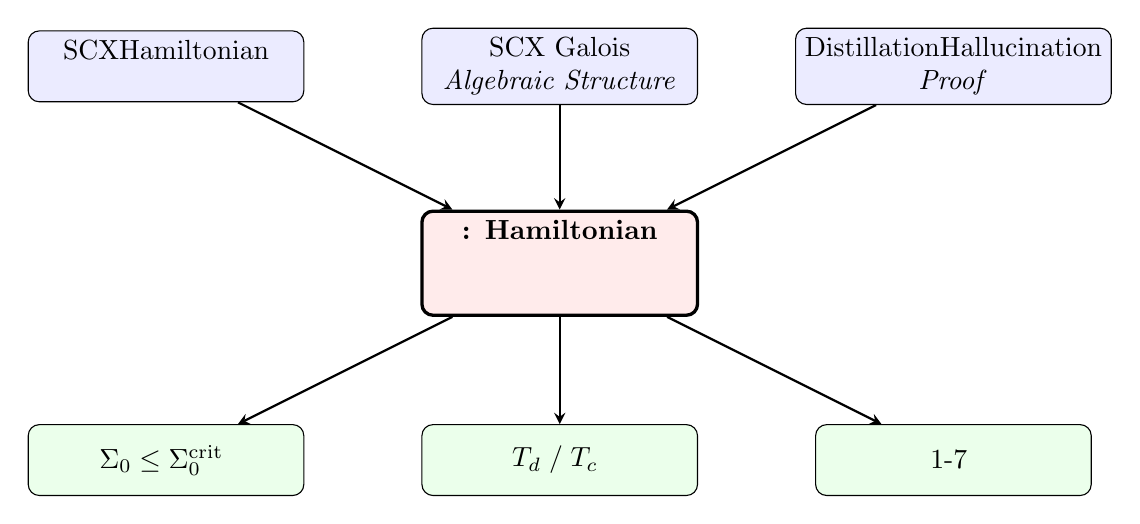
\begin{tikzpicture}[
    theory/.style={draw,rounded corners,minimum width=3.5cm,minimum height=0.9cm,align=center,fill=blue!8},
    tool/.style={draw,rounded corners,minimum width=3.5cm,minimum height=0.9cm,align=center,fill=green!8},
    diagnosis/.style={draw,rounded corners,minimum width=3.5cm,minimum height=0.9cm,align=center,fill=red!8,very thick},
    arrow/.style={->,>=stealth,thick}
]
    % Top row: foundations
    \node[theory] (hamiltonian) at (0,0) {
        SCXHamiltonian\\
        \textit{}
    };
    \node[theory] (galois) at (5,0) {
        SCX Galois\\
        \textit{Algebraic Structure}
    };
    \node[theory] (distill) at (10,0) {
        DistillationHallucination\\
        \textit{Proof}
    };
    % Middle: this paper
    \node[diagnosis] (this) at (5,-2.5) {
        \textbf{: Hamiltonian}\\
        \textit{}\\
    };
    % Bottom: outputs
    \node[tool] (auditcond) at (0,-5) {
        $\Sigma_0 \leq \Sigma_0^{\text{crit}}$
    };
    \node[tool] (phase) at (5,-5) {
        $T_d\;/\;T_c$
    };
    \node[tool] (protocol) at (10,-5) {
        1-7
    };
    % Arrows
    \draw[arrow] (hamiltonian) -- (this);
    \draw[arrow] (galois) -- (this);
    \draw[arrow] (distill) -- (this);
    \draw[arrow] (this) -- (auditcond);
    \draw[arrow] (this) -- (phase);
    \draw[arrow] (this) -- (protocol);
    % Labels
    \node[font=\footnotesize,text=blue!60] at (2.5,-1.2) {};
    \node[font=\footnotesize,text=blue!60] at (6.5,-1.2) {};
    \node[font=\footnotesize,text=blue!60] at (9,-1.2) {};
\end{tikzpicture}
\caption{SCXTheoretical System.:}
\label{fig:theory_map}
\end{figure}
\subsection{}
\begin{enumerate}[label=(\arabic*),itemsep=3pt]
    \item \textbf{: } SCX, Hamiltonian(~\ref{prot:diagnosis}).
    \item \textbf{: } """", 
    \item \textbf{Distillation: } Distillation(Distillation), 
    Distillation$\fRSB$\textbf{}---SCX.
    \item \textbf{: } (, RLHF, Distillation), 
    $\RS$$\oneRSB$$\fRSB$.
\end{enumerate}
% ================================================================
% 9. Conclusion
% ================================================================
\section{Conclusion}
SCXHamiltonian\textbf{}.
CoreConclusion: 
\begin{enumerate}[label=(\arabic*),itemsep=3pt]
    \item \textbf{: } , $\Sigma_0$---
    $\Auditable(\text{claim}) \Longleftrightarrow \Sigma_0 \leq \frac{1}{N}\log(M_{\text{feasible}}/C)$.
    \item \textbf{Parisi: } $\RS$()$\to$ $\oneRSB$()$\to$ $\fRSB$(Galois)
    $\Sigma_0$.
    \item \textbf{: } , .
    \item \textbf{Distillation: } Distillation$\RS$$\fRSB$---
    \item \textbf{: } SCX.
\end{enumerate}
, \textbf{}.
\subsection*{Acknowledgments}
 Giorgio Parisi(2021) Marc Mézard, Miguel Virasoro 
% ================================================================
% References
% ================================================================
\begin{thebibliography}{99}
\bibitem{scx_hamiltonian}
SCX.
\emph{HamiltonianSCX: }.
Preprint, 2026.
\bibitem{scx_galois}
SCX.
\emph{Galois-SCX: }.
Preprint, 2026.
\bibitem{scx_galois_falsifiability}
SCX.
\emph{Galois: SCX}.
Preprint, 2026.
\bibitem{scx_distillation_hallucination}
SCX.
\emph{Hallucination---CompactnessGaloisDistillation}.
Preprint, 2026.
\bibitem{scx_agentic}
SCX.
\emph{Agentic Multi-Agent SCX: Agentic Audit}.
Preprint, 2026.
\bibitem{parisi1979}
G.~Parisi.
``Infinite number of order parameters for spin-glasses,''
\emph{Phys. Rev. Lett.}, vol.~43, pp.~1754--1756, 1979.
\bibitem{parisi1980}
G.~Parisi.
``A sequence of approximated solutions to the S-K model for spin glasses,''
\emph{J. Phys. A: Math. Gen.}, vol.~13, pp.~L115--L121, 1980.
\bibitem{mezard1987}
M.~M\'ezard, G.~Parisi, and M.~A.~Virasoro.
\emph{Spin Glass Theory and Beyond}.
World Scientific, Singapore, 1987.
\bibitem{derrida1986}
B.~Derrida and H.~Spohn.
``Polymers on disordered trees, spin glasses, and traveling waves,''
\emph{J. Stat. Phys.}, vol.~51, pp.~817--840, 1988.
\bibitem{fyodorov2004}
Y.~V.~Fyodorov.
``Complexity of random energy landscapes, glass transition, and absolute value of the spectral determinant of random matrices,''
\emph{Phys. Rev. Lett.}, vol.~92, p.~240601, 2004.
\bibitem{hinton2015distilling}
G.~Hinton, O.~Vinyals, and J.~Dean.
``Distilling the knowledge in a neural network,''
\emph{NeurIPS Deep Learning Workshop}, 2014.
\bibitem{choromanska2015}
A.~Choromanska, M.~Henaff, M.~Mathieu, G.~Ben Arous, and Y.~LeCun.
``The loss surfaces of multilayer networks,''
in \emph{Proc. AISTATS}, 2015, pp.~192--204.
\bibitem{baity2019}
M.~Baity-Jesi, L.~Sagun, M.~Geiger, S.~Spigler, G.~Ben Arous, C.~Cammarota, Y.~LeCun, and M.~Wyart.
``Comparing dynamics: Deep neural networks versus glassy systems,''
\emph{J. Stat. Mech.}, vol.~2019, p.~124013, 2019.
\bibitem{castellani2005}
T.~Castellani and A.~Cavagna.
``Spin-glass theory for pedestrians,''
\emph{J. Stat. Mech.}, vol.~2005, p.~P05012, 2005.
\bibitem{talagrand2003}
M.~Talagrand.
\emph{Spin Glasses: A Challenge for Mathematicians}.
Springer, Berlin, 2003.
\bibitem{guerra2003}
F.~Guerra.
``Broken replica symmetry bounds in the mean field spin glass model,''
\emph{Comm. Math. Phys.}, vol.~233, pp.~1--12, 2003.
\bibitem{dauphin2014}
Y.~Dauphin, R.~Pascanu, C.~Gulcehre, K.~Cho, S.~Ganguli, and Y.~Bengio.
``Identifying and attacking the saddle point problem in high-dimensional non-convex optimization,''
in \emph{Proc. NeurIPS}, 2014, pp.~2933--2941.
\bibitem{geiger2020}
M.~Geiger, S.~Spigler, S.~d'Ascoli, L.~Sagun, M.~Baity-Jesi, G.~Biroli, and M.~Wyart.
``Jamming transition as a paradigm to understand the loss landscape of deep neural networks,''
\emph{Phys. Rev. E}, vol.~101, p.~012115, 2020.
\bibitem{sagun2017}
L.~Sagun, L.~Bottou, and Y.~LeCun.
``Eigenvalues of the Hessian in deep learning: Singularity and beyond,''
in \emph{Proc. ICLR Workshop}, 2017.
\bibitem{jacot2018}
A.~Jacot, F.~Gabriel, and C.~Hongler.
``Neural tangent kernel: Convergence and generalization in neural networks,''
in \emph{Proc. NeurIPS}, 2018, pp.~8571--8580.
\end{thebibliography}
\end{document}
